
\documentclass[letterpaper,hide notes,xcolor={table,svgnames},pdftex]{beamer}
\def\showexamples{t}


%\usepackage[svgnames]{xcolor}

%% Demo talk
%\documentclass[letterpaper,notes=show]{beamer}

\usecolortheme{crane}
\setbeamertemplate{navigation symbols}{}

\usetheme{MyPittsburgh}
%\usetheme{Frankfurt}

%\usepackage{tipa}

\usepackage{hyperref}
\usepackage{graphicx,xspace}
\usepackage[normalem]{ulem}

\newcommand\SF[1]{$\bigstar$\footnote{SF: #1}}



\newcounter{tmpnumSlide}
\newcounter{tmpnumNote}

% old question code
%\newcommand\question[1]{{$\bigstar$ \small \onlySlide{2}{#1}}}
% \newcommand\nquestion[1]{\ifdefined \presentationonly \textcircled{?} \fi \note{\par{\Large \textbf{?}} #1}}
% \newcommand\nanswer[1]{\note{\par{\Large \textbf{A}} #1}}


 \newcommand\mnote[1]{%
   \addtocounter{tmpnumSlide}{1}
   \ifdefined\showcues {~\tiny\fbox{\arabic{tmpnumSlide}}}\fi
   \note{\setlength{\parskip}{1ex}\addtocounter{tmpnumNote}{1}\textbf{\Large \arabic{tmpnumNote}:} {#1\par}}}

\newcommand\mmnote[1]{\note{\setlength{\parskip}{1ex}#1\par}}

%\newcommand\mnote[2][]{\ifdefined\handoutwithnotes {~\tiny\fbox{#1}}\fi
% \note{\setlength{\parskip}{1ex}\textbf{\Large #1:} #2\par}}

%\newcommand\mnote[2][]{{\tiny\fbox{#1}} \note{\setlength{\parskip}{1ex}\textbf{\Large #1:} #2\par}}

\newcommand\mquestion[2]{{~\color{red}\fbox{?}}\note{\setlength{\parskip}{1ex}\par{\Large \textbf{?}} #1} \note{\setlength{\parskip}{1ex}\par{\Large \textbf{A}} #2\par}\ifdefined \presentationonly \pause \fi}

\newcommand\blackboard[1]{%
\ifdefined   \showblackboard
  {#1}
  \else {\begin{center} \fbox{\colorbox{blue!30}{%
         \begin{minipage}{.95\linewidth}%
           \hspace{\stretch{1}} Some space intentionally left blank; done at the blackboard.%
         \end{minipage}}}\end{center}}%
         \fi%
}



%\newcommand\q{\tikz \node[thick,color=black,shape=circle]{?};}
%\newcommand\q{\ifdefined \presentationonly \textcircled{?} \fi}

\usepackage{listings}
\lstset{%
  keywordstyle=\bfseries,
  aboveskip=15pt,
  belowskip=15pt,
  captionpos=b,
  identifierstyle=\ttfamily,
  escapeinside={(*@}{@*)},
  stringstyle=\ttfamiliy,
  frame=lines,
  numbers=left, basicstyle=\scriptsize, numberstyle=\tiny, stepnumber=0, numbersep=2pt}

\usepackage{siunitx}
\newcommand\sius[1]{\num[group-separator = {,}]{#1}\si{\micro\second}}
\newcommand\sims[1]{\num[group-separator = {,}]{#1}\si{\milli\second}}
\newcommand\sins[1]{\num[group-separator = {,}]{#1}\si{\nano\second}}
\sisetup{group-separator = {,}, group-digits = true}

%% -------------------- tikz --------------------
\usepackage{tikz}
\usetikzlibrary{positioning}
\usetikzlibrary{arrows,backgrounds,automata,decorations.shapes,decorations.pathmorphing,decorations.markings,decorations.text}

\tikzstyle{place}=[circle,draw=blue!50,fill=blue!20,thick, inner sep=0pt,minimum size=6mm]
\tikzstyle{transition}=[rectangle,draw=black!50,fill=black!20,thick, inner sep=0pt,minimum size=4mm]

\tikzstyle{block}=[rectangle,draw=black, thick, inner sep=5pt]
\tikzstyle{bullet}=[circle,draw=black, fill=black, thin, inner sep=2pt]

\tikzstyle{pre}=[<-,shorten <=1pt,>=stealth',semithick]
\tikzstyle{post}=[->,shorten >=1pt,>=stealth',semithick]
\tikzstyle{bi}=[<->,shorten >=1pt,shorten <=1pt, >=stealth',semithick]

\tikzstyle{mut}=[-,>=stealth',semithick]

\tikzstyle{treereset}=[dashed,->, shorten >=1pt,>=stealth',thin]

\usepackage{ifmtarg}
\usepackage{xifthen}
\makeatletter
% new counter to now which frame it is within the sequence
\newcounter{multiframecounter}
% initialize buffer for previously used frame title
\gdef\lastframetitle{\textit{undefined}}
% new environment for a multi-frame
\newenvironment{multiframe}[1][]{%
\ifthenelse{\isempty{#1}}{%
% if no frame title was set via optional parameter,
% only increase sequence counter by 1
\addtocounter{multiframecounter}{1}%
}{%
% new frame title has been provided, thus
% reset sequence counter to 1 and buffer frame title for later use
\setcounter{multiframecounter}{1}%
\gdef\lastframetitle{#1}%
}%
% start conventional frame environment and
% automatically set frame title followed by sequence counter
\begin{frame}%
\frametitle{\lastframetitle~{\normalfont(\arabic{multiframecounter})}}%
}{%
\end{frame}%
}
\makeatother

\makeatletter
\newdimen\tu@tmpa%
\newdimen\ydiffl%
\newdimen\xdiffl%
\newcommand\ydiff[2]{%
    \coordinate (tmpnamea) at (#1);%
    \coordinate (tmpnameb) at (#2);%
    \pgfextracty{\tu@tmpa}{\pgfpointanchor{tmpnamea}{center}}%
    \pgfextracty{\ydiffl}{\pgfpointanchor{tmpnameb}{center}}%
    \advance\ydiffl by -\tu@tmpa%
}
\newcommand\xdiff[2]{%
    \coordinate (tmpnamea) at (#1);%
    \coordinate (tmpnameb) at (#2);%
    \pgfextractx{\tu@tmpa}{\pgfpointanchor{tmpnamea}{center}}%
    \pgfextractx{\xdiffl}{\pgfpointanchor{tmpnameb}{center}}%
    \advance\xdiffl by -\tu@tmpa%
}
\makeatother
\newcommand{\copyrightbox}[3][r]{%
\begin{tikzpicture}%
\node[inner sep=0pt,minimum size=2em](ciimage){#2};
\usefont{OT1}{phv}{n}{n}\fontsize{4}{4}\selectfont
\ydiff{ciimage.south}{ciimage.north}
\xdiff{ciimage.west}{ciimage.east}
\ifthenelse{\equal{#1}{r}}{%
\node[inner sep=0pt,right=1ex of ciimage.south east,anchor=north west,rotate=90]%
{\raggedleft\color{black!50}\parbox{\the\ydiffl}{\raggedright{}#3}};%
}{%
\ifthenelse{\equal{#1}{l}}{%
\node[inner sep=0pt,right=1ex of ciimage.south west,anchor=south west,rotate=90]%
{\raggedleft\color{black!50}\parbox{\the\ydiffl}{\raggedright{}#3}};%
}{%
\node[inner sep=0pt,below=1ex of ciimage.south west,anchor=north west]%
{\raggedleft\color{black!50}\parbox{\the\xdiffl}{\raggedright{}#3}};%
}
}
\end{tikzpicture}
}


%% --------------------

%\usepackage[excludeor]{everyhook}
%\PushPreHook{par}{\setbox0=\lastbox\llap{MUH}}\box0}

%\vspace*{\stretch{1}

%\setbox0=\lastbox \llap{\textbullet\enskip}\box0}

\setlength{\parskip}{\fill}

\newcommand\noskips{\setlength{\parskip}{1ex}}
\newcommand\doskips{\setlength{\parskip}{\fill}}

\newcommand\xx{\par\vspace*{\stretch{1}}\par}
\newcommand\xxs{\par\vspace*{2ex}\par}
\newcommand\tuple[1]{\langle #1 \rangle}
\newcommand\code[1]{{\sf \footnotesize #1}}
\newcommand\ex[1]{\uline{Example:} \ifdefined \presentationonly \pause \fi
  \ifdefined\showexamples#1\xspace\else{\uline{\hspace*{2cm}}}\fi}

\newcommand\ceil[1]{\lceil #1 \rceil}


\AtBeginSection[]
{
   \begin{frame}
       \frametitle{Outline}
       \tableofcontents[currentsection]
   \end{frame}
}



\pgfdeclarelayer{edgelayer}
\pgfdeclarelayer{nodelayer}
\pgfsetlayers{edgelayer,nodelayer,main}

\tikzstyle{none}=[inner sep=0pt]
\tikzstyle{rn}=[circle,fill=Red,draw=Black,line width=0.8 pt]
\tikzstyle{gn}=[circle,fill=Lime,draw=Black,line width=0.8 pt]
\tikzstyle{yn}=[circle,fill=Yellow,draw=Black,line width=0.8 pt]
\tikzstyle{empty}=[circle,fill=White,draw=Black]
\tikzstyle{bw} = [rectangle, draw, fill=blue!20, 
    text width=4em, text centered, rounded corners, minimum height=2em]
    
    \newcommand{\CcNote}[1]{% longname
	This work is licensed under the \textit{Creative Commons #1 3.0 License}.%
}
\newcommand{\CcImageBy}[1]{%
	\includegraphics[scale=#1]{creative_commons/cc_by_30.pdf}%
}
\newcommand{\CcImageSa}[1]{%
	\includegraphics[scale=#1]{creative_commons/cc_sa_30.pdf}%
}
\newcommand{\CcImageNc}[1]{%
	\includegraphics[scale=#1]{creative_commons/cc_nc_30.pdf}%
}
\newcommand{\CcGroupBySa}[2]{% zoom, gap
	\CcImageBy{#1}\hspace*{#2}\CcImageNc{#1}\hspace*{#2}\CcImageSa{#1}%
}
\newcommand{\CcLongnameByNcSa}{Attribution-NonCommercial-ShareAlike}

\newenvironment{changemargin}[1]{% 
  \begin{list}{}{% 
    \setlength{\topsep}{0pt}% 
    \setlength{\leftmargin}{#1}% 
    \setlength{\rightmargin}{1em}
    \setlength{\listparindent}{\parindent}% 
    \setlength{\itemindent}{\parindent}% 
    \setlength{\parsep}{\parskip}% 
  }% 
  \item[]}{\end{list}} 




\title{Lecture 30 --- Software Bricolage}

\author{Patrick Lam \& Jeff Zarnett\\ \small \texttt{p.lam@ece.uwaterloo.ca} \& \texttt{jzarnett@uwaterloo.ca}}
\institute{Department of Electrical and Computer Engineering \\[-1ex]
  University of Waterloo}
\date{\today}

\begin{document}

\begin{frame}
  \titlepage

  \vfill
  \begin{center}
    \CcGroupBySa{0.83}{0.95ex}\\
                  {\tiny\CcNote{\CcLongnameByNcSa}}
                  \vspace*{-2.5ex}
  \end{center}

\end{frame}

\part{Software Bricolage}
\frame{\partpage}

\begin{frame}
\frametitle{Software Bricolage}
\begin{changemargin}{1cm}
\Large

Today: Assignments vs real-world programming.\\[1em]

Most of your work for school is not open-ended until FYDP.\\[1em]

Some of your work in co-op will be open-ended. We'll see techniques 
for doing this work.
\end{changemargin}

\end{frame}

\begin{frame}
\frametitle{Schoolwork}

\begin{center}
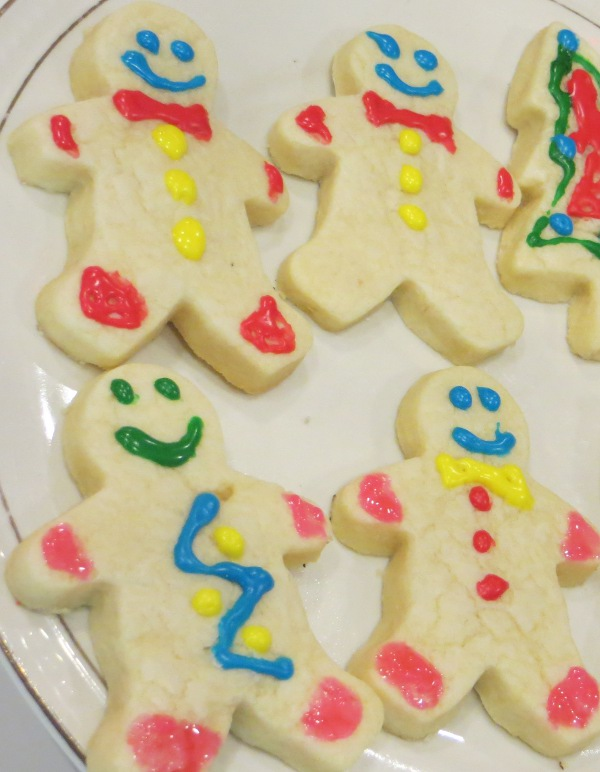
\includegraphics[width=.4\textwidth]{images/1502_cookies}
\end{center}

\begin{changemargin}{1cm}
Ideally:
\begin{itemize}
\item well-specified
\item we provide tools and libraries you'll need (e.g.~{\tt LineGraphView}).
\end{itemize}
\end{changemargin}

\end{frame}

\begin{frame}
\frametitle{More on schoolwork}

\begin{changemargin}{1.5cm}
We have educational goals, so you get:
\begin{itemize}
\item Lots of template code---you fill in the blanks.
\item Problems you can solve cleanly in a single language (Java).
\end{itemize}

e.g. Assignment 4: less than 50 lines; my Lab 1: 110 lines.\\[1em]

By the way, if you want to do an open-ended project for Labs 3 and 4,
talk to me.

\end{changemargin}

\end{frame}

\begin{frame}
\frametitle{Real-world Programming}

\Large
\begin{changemargin}{2cm}
Often: check out large codebase, \\ \qquad fix~something.\\[1em]

Sometimes: start a project from scratch.\\
\qquad (But not really from scratch).
\end{changemargin}
\end{frame}

\begin{frame}
\frametitle{Getting Started}

\begin{changemargin}{1cm}
\Large
You have a goal.\\[1em]

Need to formalize the goal:
\begin{itemize}
\item even high-quality software is no good unless it meets requirements.
\end{itemize}
~\\[1em]
ECE451 is all about requirements.
\end{changemargin}

\end{frame}

\begin{frame}
\frametitle{Steps to Build Software (per Philip Guo)}

\begin{changemargin}{1cm}
\Huge
\begin{enumerate}
\item Forage
\item Tinker
\item Weld
\item Grow
\item Doubt
\item Refactor
\end{enumerate}
\end{changemargin}

\end{frame}

\begin{frame}

\frametitle{Step 1: Foraging}

\begin{center}
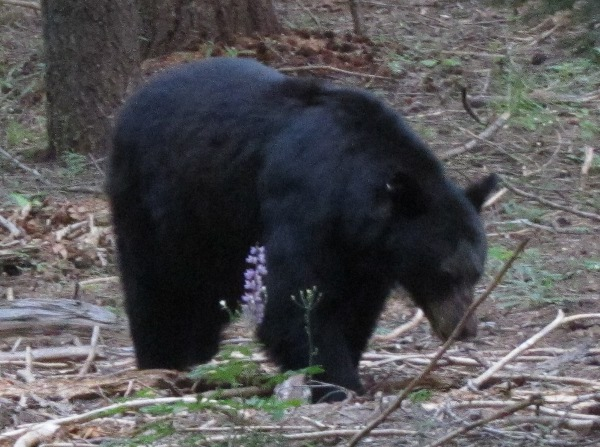
\includegraphics[width=.4\textwidth]{images/0673_foraging}
\end{center}
{\tiny \hfill (P. Lam collection)}

\begin{changemargin}{1cm}
Look for suitable components/libraries.\\
\qquad (maybe yours, maybe others').\\
\qquad Know what's out there.\\[1em]

It may be documented (if you're lucky).\\[1em]

Components may be in different languages.

\end{changemargin}

\end{frame}

\begin{frame}

\frametitle{Step 2: Tinker}

\begin{tabular}{cc}
\begin{minipage}{.35 \textwidth}
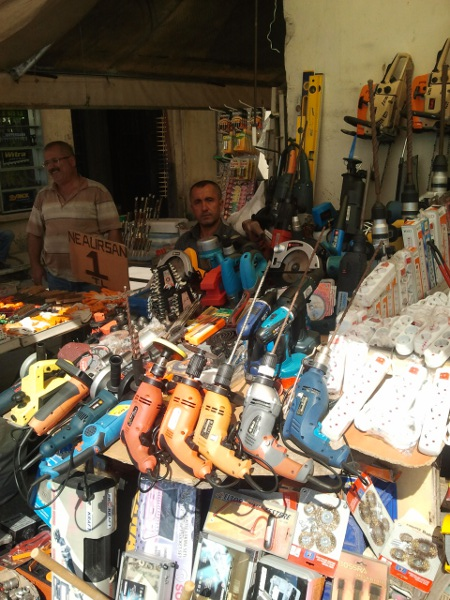
\includegraphics[width=\textwidth]{images/home_hardware}\\
{\tiny \hspace*{.5\textwidth} (P. Lam collection)}
\end{minipage}&
\begin{minipage}{.6\textwidth}
\begin{itemize}
\item What can your code actually do?
\item Experiment with the software! 
\item Give it test inputs.
\item Instrument the code. Modify it.
\end{itemize}
This is very much like debugging.\\[1em]

Repeat foraging and tinkering as needed.
\end{minipage}
\end{tabular}

\end{frame}

\begin{frame}
\frametitle{Step 3: Weld}
\begin{changemargin}{2cm}
\Large
Two potential problems:
\begin{itemize}
\item dependencies;
\item impedence mismatches.
\end{itemize}
\end{changemargin}
\end{frame}

\begin{frame}
\frametitle{Dependencies}

\begin{center}
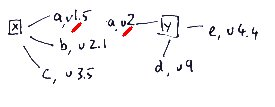
\includegraphics[width=.8\textwidth]{images/dependencies}
\end{center}

\begin{changemargin}{1.5cm}
\Large
Sometimes you can't get version you need.\\[1em]
Sometimes required versions conflict.
\end{changemargin}

\end{frame}

\begin{frame}
\frametitle{Impedence mismatches}

\begin{center}
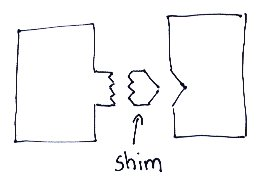
\includegraphics[width=.7\textwidth]{images/shim}
\end{center}

\begin{changemargin}{2cm}
\Large
\item You may have to build a shim\\ \qquad (e.g. XML output, CSV input!)
\end{changemargin}

\end{frame}

\begin{frame}
\frametitle{Step 4: Grow}
\begin{changemargin}{1.5cm}
\Large
Start building code.\\[1em]
Begin with simple examples, concrete code.\\[1em]
What's the simplest thing that can work?\\[1em]
Challenge: fix bad welds.
\end{changemargin}
\end{frame}

\begin{frame}
\frametitle{Step 5: Doubt}

\Large
\begin{changemargin}{2cm}
\begin{itemize}
\item Don't reinvent the wheel.\\
 Know what's in libraries.\\
 Ask the authors.\\
 Contribute to the library.
\end{itemize}
\end{changemargin}

\end{frame}

\begin{frame}
\frametitle{Step 6: Refactor}

\Large
\begin{changemargin}{2cm}
Clean your code, make it more general.\\[1em]
Improve interactions between your code and others.
\end{changemargin}

\end{frame}

\begin{frame}
\frametitle{Iterate}

\begin{changemargin}{1cm}
\Large
Iterate steps 4--6 as needed.\\
Grow, doubt, refactor.
\end{changemargin}
\end{frame}

\begin{frame}
\frametitle{Using the Web for Programming}

\begin{changemargin}{1cm}
Beware: Don't indiscriminately copy code from the Internet.\\
Policy 71, and lawsuits (in industry).\\[1em]

Highly useful when used properly.
\end{changemargin}

\end{frame}

\begin{frame}
\frametitle{Three Main Ways}

\Large
\begin{changemargin}{2cm}
\begin{itemize}
\item Learn concepts.
\item Clarify existing knowledge.
\item Remind of details.
\end{itemize}
\end{changemargin}
\end{frame}

\begin{frame}
\frametitle{Learning concepts}

\Large
\begin{changemargin}{1.5cm}
\item Read tutorials.\\
Slow; hard to find good ones.\\
Gives an understanding of how things work.
\item Experiment with sample code.
\end{changemargin}
\end{frame}


\begin{frame}
\frametitle{Clarify existing knowledge}

\begin{changemargin}{2cm}
\Large
\begin{itemize}
\item Have some existing knowledge.
\item Not quite sure about it.
\item Also look up error messages (stackoverflow).
\end{itemize}
\end{changemargin}

\end{frame}

\begin{frame}
\frametitle{Remind of details}

\Large
\begin{changemargin}{1cm}
\begin{itemize}
\item especially syntax: not that important.
\end{itemize}

General tip: refine your queries iteratively.
\end{changemargin}
\end{frame}

\part{Licensing}
\frame{\partpage}

\begin{frame}
\frametitle{Software Licenses}

\begin{changemargin}{1cm}
A \alert{Software License} is a legal instrument that tells us how a piece of software may be used or distributed.

It grants you the rights to do things that would otherwise be an infringement (violation) of copyright law.


\end{changemargin}
\end{frame}

\begin{frame}
\frametitle{Software Licenses}

\begin{changemargin}{1cm}

Answers questions like:

\begin{itemize}
	\item Where, how \& how often can you install the program?
	\item Can you copy, modify, or redistribute it?
	\item Can you look at the underlying source code?
\end{itemize}

\end{changemargin}
\end{frame}


\begin{frame}
\frametitle{Software Licenses: Ignore Them?}

\begin{changemargin}{1cm}

This is boring. Who cares?! We do - can't ignore it.

If you do not explicitly declare a license, you effectively get one anyway. 

Code, like other works, is automatically copyrighted by default.

People can read code, but they have no legal right to use it.
\end{changemargin}
\end{frame}

\begin{frame}
\frametitle{Software Licenses: Proprietary}

\begin{changemargin}{1cm}
Impossible to generalize.

You get the rights specified in the license and that's it.

\end{changemargin}
\end{frame}

\begin{frame}
\frametitle{Software Licenses: GNU GPL}

\begin{changemargin}{1cm}
Most common example of an open-source license.

Referred to as ``Copyleft''.

Ensures code can be used, copied, modified, and redistributed.

Code under this license can't be used in proprietary programs.

Any changes you make must be licensed under GPL.

\end{changemargin}
\end{frame}


\begin{frame}
\frametitle{Software Licenses: GNU GPLv2 \& GPLv3}

\begin{changemargin}{1cm}
More recent update to the GPL: version 3.

Intended to address a shortcoming called \alert{Tivoization}.

Named after the Tivo digital video recorder.

\end{changemargin}
\end{frame}

\begin{frame}
\frametitle{Software Licenses: GNU GPLv2 \& GPLv3}
\begin{center}

\includegraphics[width=0.3\textwidth]{images/tivo.png}
\end{center}

Tivo was based on Linux, open source software.
 
Added hardware protection to prevent modifying the software.

\end{frame}

\begin{frame}
\frametitle{Software Licenses: GNU LGPL}

\begin{changemargin}{1cm}
The Lesser GPL is intended for software libraries.

Binary (compiled) code can be linked to proprietary programs.

Library code must follow GPL restrictions.

\end{changemargin}
\end{frame}


\begin{frame}
\frametitle{Software Licenses: BSD}

\begin{changemargin}{1cm}
A permissive open-source license.

Allows any use of code, even making it a proprietary product.

Disclaims all liability.

No requirement to share changes under any license.

\end{changemargin}
\end{frame}

\begin{frame}
\frametitle{Software Licenses: Mozilla}

\begin{changemargin}{1cm}
Open source license from the people who make Firefox.

Allows source code to be mixed - open-source + proprietary.

Any file licensed under MPL must be open source;\\
\quad But not all files must be open-sourced.

Hybrid between BSD and GPL licenses.

\end{changemargin}
\end{frame}

\begin{frame}
\frametitle{Software Licenses: Public Domain}

\begin{changemargin}{1cm}
No copyright owner - may be used by anyone for any purpose.

All copyrighted works will eventually enter the public domain.\\
\quad\quad But this can take a long time. Life + 70 years.

Authors can explicitly put code in the public domain.

\end{changemargin}
\end{frame}

\begin{frame}
\frametitle{Software Licenses: Public Domain}

\begin{changemargin}{1cm}
In the USA the amount of time before work enters the public domain keeps getting extended.

Disney is a big advocate: want to keep Steamboat Willie (first Mickey Mouse animation) from entering the public domain.

\end{changemargin}
\end{frame}

\begin{frame}
\frametitle{Software Licenses: Public Domain}

\begin{changemargin}{1cm}

\begin{center}
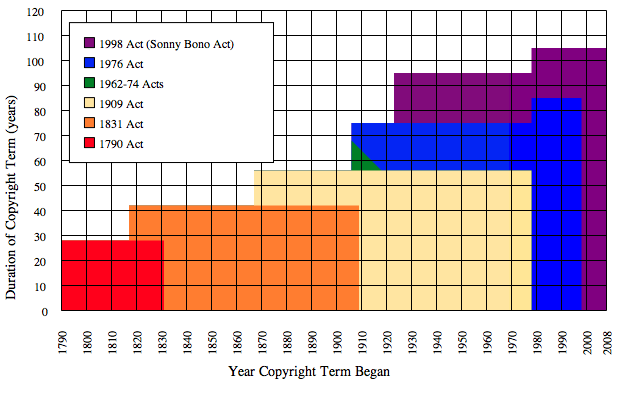
\includegraphics[width=0.75\textwidth]{images/copyright-term.png}
\end{center}

You may safely assume a work will never enter the public domain unless the author chooses to put it there.

\end{changemargin}
\end{frame}


\begin{frame}
\frametitle{License Violations}

\begin{changemargin}{1cm}

License violations are taken seriously and lead to legal action.

Importing open source code into your software can get you into a lot of trouble.

\end{changemargin}
\end{frame}



\begin{frame}
\frametitle{License Violation Example}

\begin{changemargin}{1cm}

Landgericht Hamburg found a company, FANTEC, guilty of violating the GPL in their media player.

They distributed their firmware, containing some software licensed under the GPL (\texttt{iptables}).

They did not distribute the code as the GPL requires.

The court required FANTEC to pay penalty fee \& legal costs.


\end{changemargin}
\end{frame}


\end{document}
